\documentclass{article}

%überschreibe command, damit arial als schriftart eingebunden werden kann
\renewcommand*{\familydefault}{\sfdefault}

%packages
\usepackage{hyperref}
\usepackage[ngerman]{babel}
\usepackage[utf8]{inputenc}
\usepackage[T1]{fontenc}
\usepackage[scaled]{uarial}
\usepackage[left=2cm,right=2cm]{geometry}
\usepackage{graphicx}
\usepackage{eurosym}
\usepackage{amsmath}
\usepackage[backend=biber]{biblatex}

% Metadaten über den autor

%farben setup für links
\hypersetup{
    colorlinks=true,
    linkcolor=black,
    filecolor=magenta,      
    urlcolor=cyan,
}

%pfad für images
\graphicspath{{img/}}

%literaturverzeichnis laden
\addbibresource{literatur.bib}


%beginn des dokuments
\begin{document}
%Deckblatt
\begin{titlepage}
\centering

\includegraphics[scale=1]{ihk.png}
\linebreak
\linebreak
\large{Abschlussprüfung Sommer 2023}
\linebreak
\linebreak
\large{Fachinformatiker für Anwendungsentwicklung}
\linebreak
\linebreak
\large{Dokumentation zur betrieblichen Projektarbeit}
\linebreak
\linebreak
\linebreak
\linebreak
\LARGE{\textbf{Entwicklung eines Zeiterfassungsmoduls für eine ERP Software}}
\\[1.5in]
\large{\textbf{Prüfungsbewerber:}}
\linebreak
\large{Vorname Nachname}
\linebreak
\large{Adresse}
\linebreak
\large{PLZ Stadt}
\\[0.5in]
\large{\textbf{Ausbildungsbetrieb:}}
\linebreak
\large{Name des Ausbildungsbetriebs}
\linebreak
\large{Adresse}
\linebreak
\large{PLZ Stadt}
\end{titlepage}

%Inhaltsverzeichnis
\newpage
\tableofcontents
\newpage

\section{Einleitung}

\subsection{Projektumfeld}

\subsection{Projektziel}

\subsection{Projektbegründung}

\subsection{Projektschnittstellen}

\subsection{Projektabgrenzung}

\section{Analyse}

\subsection{IST-Analyse}

\subsection{Wirtschaftlichkeitsanalyse}
%Leerzeichen können mit dem Tilde Zeichen (~) gesetzt werden (Alt Gr + tilde auf tastatur)
%\[ \frac{100~Euro}{200~Tage} \]

\section{Planung}

%Entwurfsphase
\section{Entwurf}

\subsection{Benutzeroberfläche}

\subsubsection{Mitarbeiterbereich}

\subsubsection{Admin Bereich}

\subsection{Datenmodell}
%mit datenmodell abbildung

\subsection{Geschäftslogik}
%darstellung der Logik des Moduls als Programmaublaufplan/Komponenten/Sequenzdiagramm
\newpage
%Implementierungsphase
\section{Implementierung}

\subsection{Implementierung der Datenstrukturen}

\subsection{Implementierung der Benutzeroberfläche}
% z.b. benutzeroberfläche mit html und css entwickelt
\subsection{Implementierung der Geschäftslogik}

\section{Validierungsphase}
%welche tests wurden durchgeführt (unit tests/ whitebox/ blackbox)

\section{Einführungsphase}
%wie lief das deployment ab (manuell/ automatisch mit pipelines)
%migration von altdaten (z.b. aus alter Zeiterfassung)
%schulungen für mitarbeiter durchgeführt?

\section{Dokumentation}
%wie wurde dokumentiert (php doc)
%anwenderdokumentation (d.h. für alle mitarbeiter, nicht nur IT leute)

\section{Fazit}

\subsection{Soll-/Ist-Vergleich}

\subsection{Gelerntes?}

\subsection{Ausblick}
%weiterentwicklung des projektes in der Zukunft

\section{Anhang}

\subsection{Abbildungsverzeichnis}

\subsubsection{Nutzwertanalyse}
%Beispiel für das Einbinden eines Bildes
\begin{center}
	\centering
	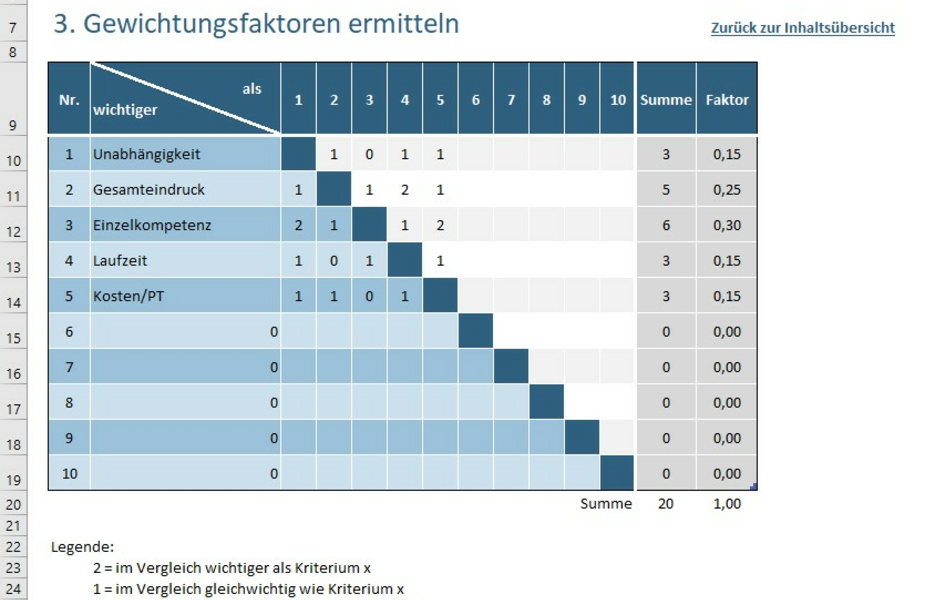
\includegraphics[scale=0.2]{nutz}
	\label{fig:nutz}
\end{center}

\subsection{Literaturverzeichnis}
Die mathematischen Beispiele stammen aus \autocite{Graham1995}.

Weitere Verweise: \parencite{Graham1995} oder \textcite{Thomas2008} oder sogar
\citetitle{Graham1995}.

\autocite[56]{Thomas2008}

\autocite[Siehe][45-48]{Graham1995}

Gemeinsam \autocite{Graham1995,Thomas2008}

\printbibliography

\end{document}


